\documentclass[10pt]{article}

% 基础包
\usepackage[UTF8]{ctex}
\usepackage[margin=2.5cm]{geometry}
\usepackage{amsmath,amssymb,amsfonts}
\usepackage{graphicx}
\usepackage{booktabs}
\usepackage{multirow}
\usepackage{array}
\usepackage{subcaption}
\usepackage{float}
\usepackage{algorithm}
\usepackage{algorithmic}
\usepackage{hyperref}
\usepackage{xcolor}
\usepackage{listings}
\usepackage{enumitem}
\usepackage{cite}

% 代码样式
\lstset{
    basicstyle=\ttfamily\small,
    breaklines=true,
    frame=single,
    language=Python
}

% 超链接设置
\hypersetup{
    colorlinks=true,
    linkcolor=blue,
    citecolor=blue,
    urlcolor=blue
}

\begin{document}

% ==================== 标题页 ====================
\title{\textbf{基于BGE和交叉注意力机制的\\
社交媒体评论热度概率预测方法}}

\author{
    李俊凯\\
    \textit{浙江工业大学信息工程学院}\\
    \texttt{302023568066@zjut.edu.cn}
}

\date{}

\maketitle

% ==================== 摘要 ====================
\begin{abstract}
社交媒体信息生态系统呈现典型的复杂适应系统特征,评论热度的生成机制内嵌着本体论层面的不确定性,传统点估计范式存在根本性局限。本文从认识论层面重新审视热度预测问题,指出其本质是对内嵌随机性的条件概率分布估计。基于此洞察,提出BGE-Attention概率预测框架:通过BGE预训练模型编码多源文本,利用Cross-Attention机制实现语义空间的条件投影;设计对数尺度负对数似然损失函数,重建误差度量的尺度不变性;提出基于MinHash的时序-语义联合特征,构建"首发-跟风"效应的可计算表达。在27万条微博评论数据上的实验表明,相比NGBoost基线,本方法将置信区间宽度(MPIW)降低六个数量级(从数千万降至3.0050),同时PICP@95\%从94.30\%提升至97.75\%,首次实现社交媒体场景下预测精度与不确定性校准的帕累托最优。代码开源于:\url{https://github.com/LJK666666666/LLM_SU7}。

\textbf{关键词:}概率预测;不确定性量化;预训练语言模型;交叉注意力机制;长尾分布建模
\end{abstract}

% ==================== 1. 引言 ====================
\section{引言}

\subsection{研究背景:复杂系统视角下的热度预测}

社交媒体已演化为一个典型的\textbf{复杂适应系统}:个体用户的微观交互行为与群体涌现的宏观传播模式相互耦合,形成跨尺度的非线性动力学\cite{liu2019sentiment}。评论热度——作为"内容-用户-平台"三元交互的投影——其生成机制内嵌着\textbf{本体论层面的不确定性}:同一语义内容在不同时序位置可产生数量级差异的传播效应。这一现象对舆情监控\cite{zhang2020brand}、品牌管理和内容推荐\cite{wu2019npa}具有重要应用价值,但也揭示了传统确定性预测范式的根本性局限。

从信息论视角审视,现有研究陷入了\textbf{"点估计陷阱"}:将本质上服从随机过程的热度演化强行映射至确定性数值空间。这不仅造成预测置信度的语义缺失,更从根本上混淆了\textbf{认知不确定性}(epistemic uncertainty,源于模型知识的不完备)与\textbf{随机不确定性}(aleatoric uncertainty,源于数据的内在随机性)的边界。

\subsection{技术挑战:三重瓶颈的系统解剖}

深入分析现有方法,我们识别出制约预测性能的三重技术瓶颈:

\textbf{(1)损失函数的尺度畸变效应}。社交媒体数据呈现典型的幂律分布(Power-law Distribution),少数评论获得海量互动,多数评论互动稀少。传统均方误差损失在此场景下表现出严重的\textbf{量纲偏倚}:对高热度样本的绝对误差过度敏感,而对低热度样本的相对误差系统性低估。这一缺陷的本质在于——欧氏距离度量未能捕捉社交媒体数据的\textbf{乘性噪声特性},即预测误差应与真实值呈比例关系而非绝对关系。

\textbf{(2)语义表征与上下文的解耦困境}。现有文本编码方案普遍采用"编码-拼接"的朴素策略,忽视了评论语义与其上下文(微博正文、父评论、根评论)之间的\textbf{条件依赖结构}。这种架构无法建模"相同评论在不同语境下热度迥异"的现象,本质上是对\textbf{语用学信息}的系统性遗漏。

\textbf{(3)时序位置效应的建模空白}。"首发效应"与"跟风效应"的热度鸿沟揭示了一个被长期忽视的先验:\textbf{文本相似性与时序先占权的交互作用}构成热度预测的关键解释变量。然而,暴力计算文本相似度的$O(n^2)$复杂度使得该特征在大规模数据上难以落地。

\subsection{本文贡献:从战术改进到范式革新}

针对上述挑战,本文提出BGE-Attention概率预测框架,实现从"点估计"到"分布预测"的\textbf{范式跃迁}。主要贡献如下:

\begin{enumerate}[leftmargin=*]
    \item \textbf{预测范式重构}:提出BGE-Attention模型,通过双预测头同时输出均值$\mu(x)$与标准差$\sigma(x)$,实现对预测值与预测置信度的联合建模,承认并显式编码预测目标的内在随机性;
    \item \textbf{损失函数的尺度不变性重建}:设计对数尺度负对数似然损失函数,通过将误差度量从原始空间映射至对数空间,实现跨量级预测误差的等权惩罚,并构建内生的不确定性正则化机制;
    \item \textbf{语义空间的条件投影}:采用Cross-Attention机制建立"评论语义-上下文语义"的条件映射关系,使评论表征从"孤立语义"升维至"情境化语义";
    \item \textbf{时序-语义联合特征空间构建}:提出基于MinHash的重复程度特征,将相似度计算复杂度从$O(n^2)$降至$O(nk)$,为"首发-跟风"效应提供可计算的数学表达。
\end{enumerate}

% ==================== 2. 相关工作 ====================
\section{相关工作}

\subsection{社交媒体热度预测:从时序建模到深度学习}

社交媒体热度预测的研究脉络经历了从统计建模到深度学习的范式演进。早期工作主要基于时间序列模型\cite{yang2011patterns},通过分析传播时序特征(如早期增长率、峰值时间)预测最终热度,其理论基础是信息传播的\textbf{马太效应}——早期获得关注的内容更易持续获得关注。Bandari等人\cite{bandari2012pulse}研究新闻文章分享预测,发现内容特征和来源对性能有显著影响,揭示了热度预测中\textbf{内容因素与渠道因素的交互作用}。

近年来,深度学习方法取得显著进展。Deng等人\cite{deng2020deep}提出基于注意力机制的神经网络模型,捕捉用户与内容的复杂交互。然而,这些方法普遍存在一个\textbf{认识论层面的局限}:仅关注点估计而忽视预测不确定性的建模。本文认为,热度预测的本质是对\textbf{条件概率分布}的估计,点估计范式无法表达模型对预测结果的置信程度。

\subsection{预训练语言模型:从词袋到上下文感知表征}

文本表征技术经历了从\textbf{符号空间}到\textbf{连续向量空间}的深刻变革。传统TF-IDF和词袋模型将文本映射为稀疏高维向量,难以捕捉词序信息和语义关系。预训练语言模型的兴起标志着NLP领域的范式革命:BERT\cite{devlin2019bert}通过掩码语言建模学习双向上下文表征,RoBERTa\cite{liu2019roberta}进一步优化了预训练策略。

BGE(BAAI General Embedding)\cite{bge2023}是面向中文的文本嵌入模型,其核心创新在于\textbf{对比学习范式}的引入——通过正负样本对的区分性训练,使语义相近的文本在嵌入空间中距离更近。本文采用BGE-base-zh-v1.5提取评论语义表示,并通过Cross-Attention机制实现\textbf{上下文感知的语义融合},使评论表征能够动态适应其所处的对话语境。

\subsection{概率预测与不确定性估计:从点估计到分布输出}

不确定性估计是机器学习中一个具有深刻理论意涵的研究方向\cite{gal2016uncertainty}。贝叶斯神经网络\cite{blundell2015weight}通过对权重施加先验分布,将参数不确定性显式建模;MC Dropout\cite{gal2016dropout}提出通过多次随机失活近似贝叶斯推断,但计算开销较大。

NGBoost\cite{duan2020ngboost}开创了\textbf{自然梯度提升}的技术路线,通过优化条件分布的参数(而非点预测值),能够直接输出预测分布。然而,该方法在社交媒体场景下面临两个挑战:(1)未针对长尾分布设计损失函数;(2)树模型难以有效利用预训练语言模型的语义表征。本文在此基础上,提出\textbf{对数尺度损失函数}重建误差度量的尺度不变性,并通过神经网络架构实现端到端的语义-数值联合建模。

% ==================== 3. 方法 ====================
\section{方法}

\subsection{问题形式化:从点估计到分布估计}

给定评论$x$及其上下文信息(所属微博、根评论、父评论)和统计特征,传统方法的目标是学习映射$f: x \mapsto \hat{y}$。本文重新定义预测目标为\textbf{条件概率分布}$P(y|x)$的估计。

基于对社交媒体数据分布特性的分析(见图\ref{fig:log_distribution}),我们假设对数变换后的热度服从正态分布:
\begin{equation}
\log(y+c) \sim \mathcal{N}(\mu(x), \sigma^2(x))
\end{equation}
其中$c$为平滑常数,$\mu(x)$和$\sigma(x)$分别为模型预测的\textbf{位置参数}(表征预测中心)和\textbf{尺度参数}(表征预测不确定性)。这一形式化的核心洞察在于:将原本隐含于预测残差中的不确定性\textbf{显式参数化},使模型能够对不同样本输出差异化的置信度。

\subsection{模型架构:多源语义的层次化融合}

本文提出的BGE-Attention模型架构如图\ref{fig:neural_networks}所示,采用\textbf{"编码-融合-预测"三阶段设计},主要包含四个功能模块。

\begin{figure}[H]
    \centering
    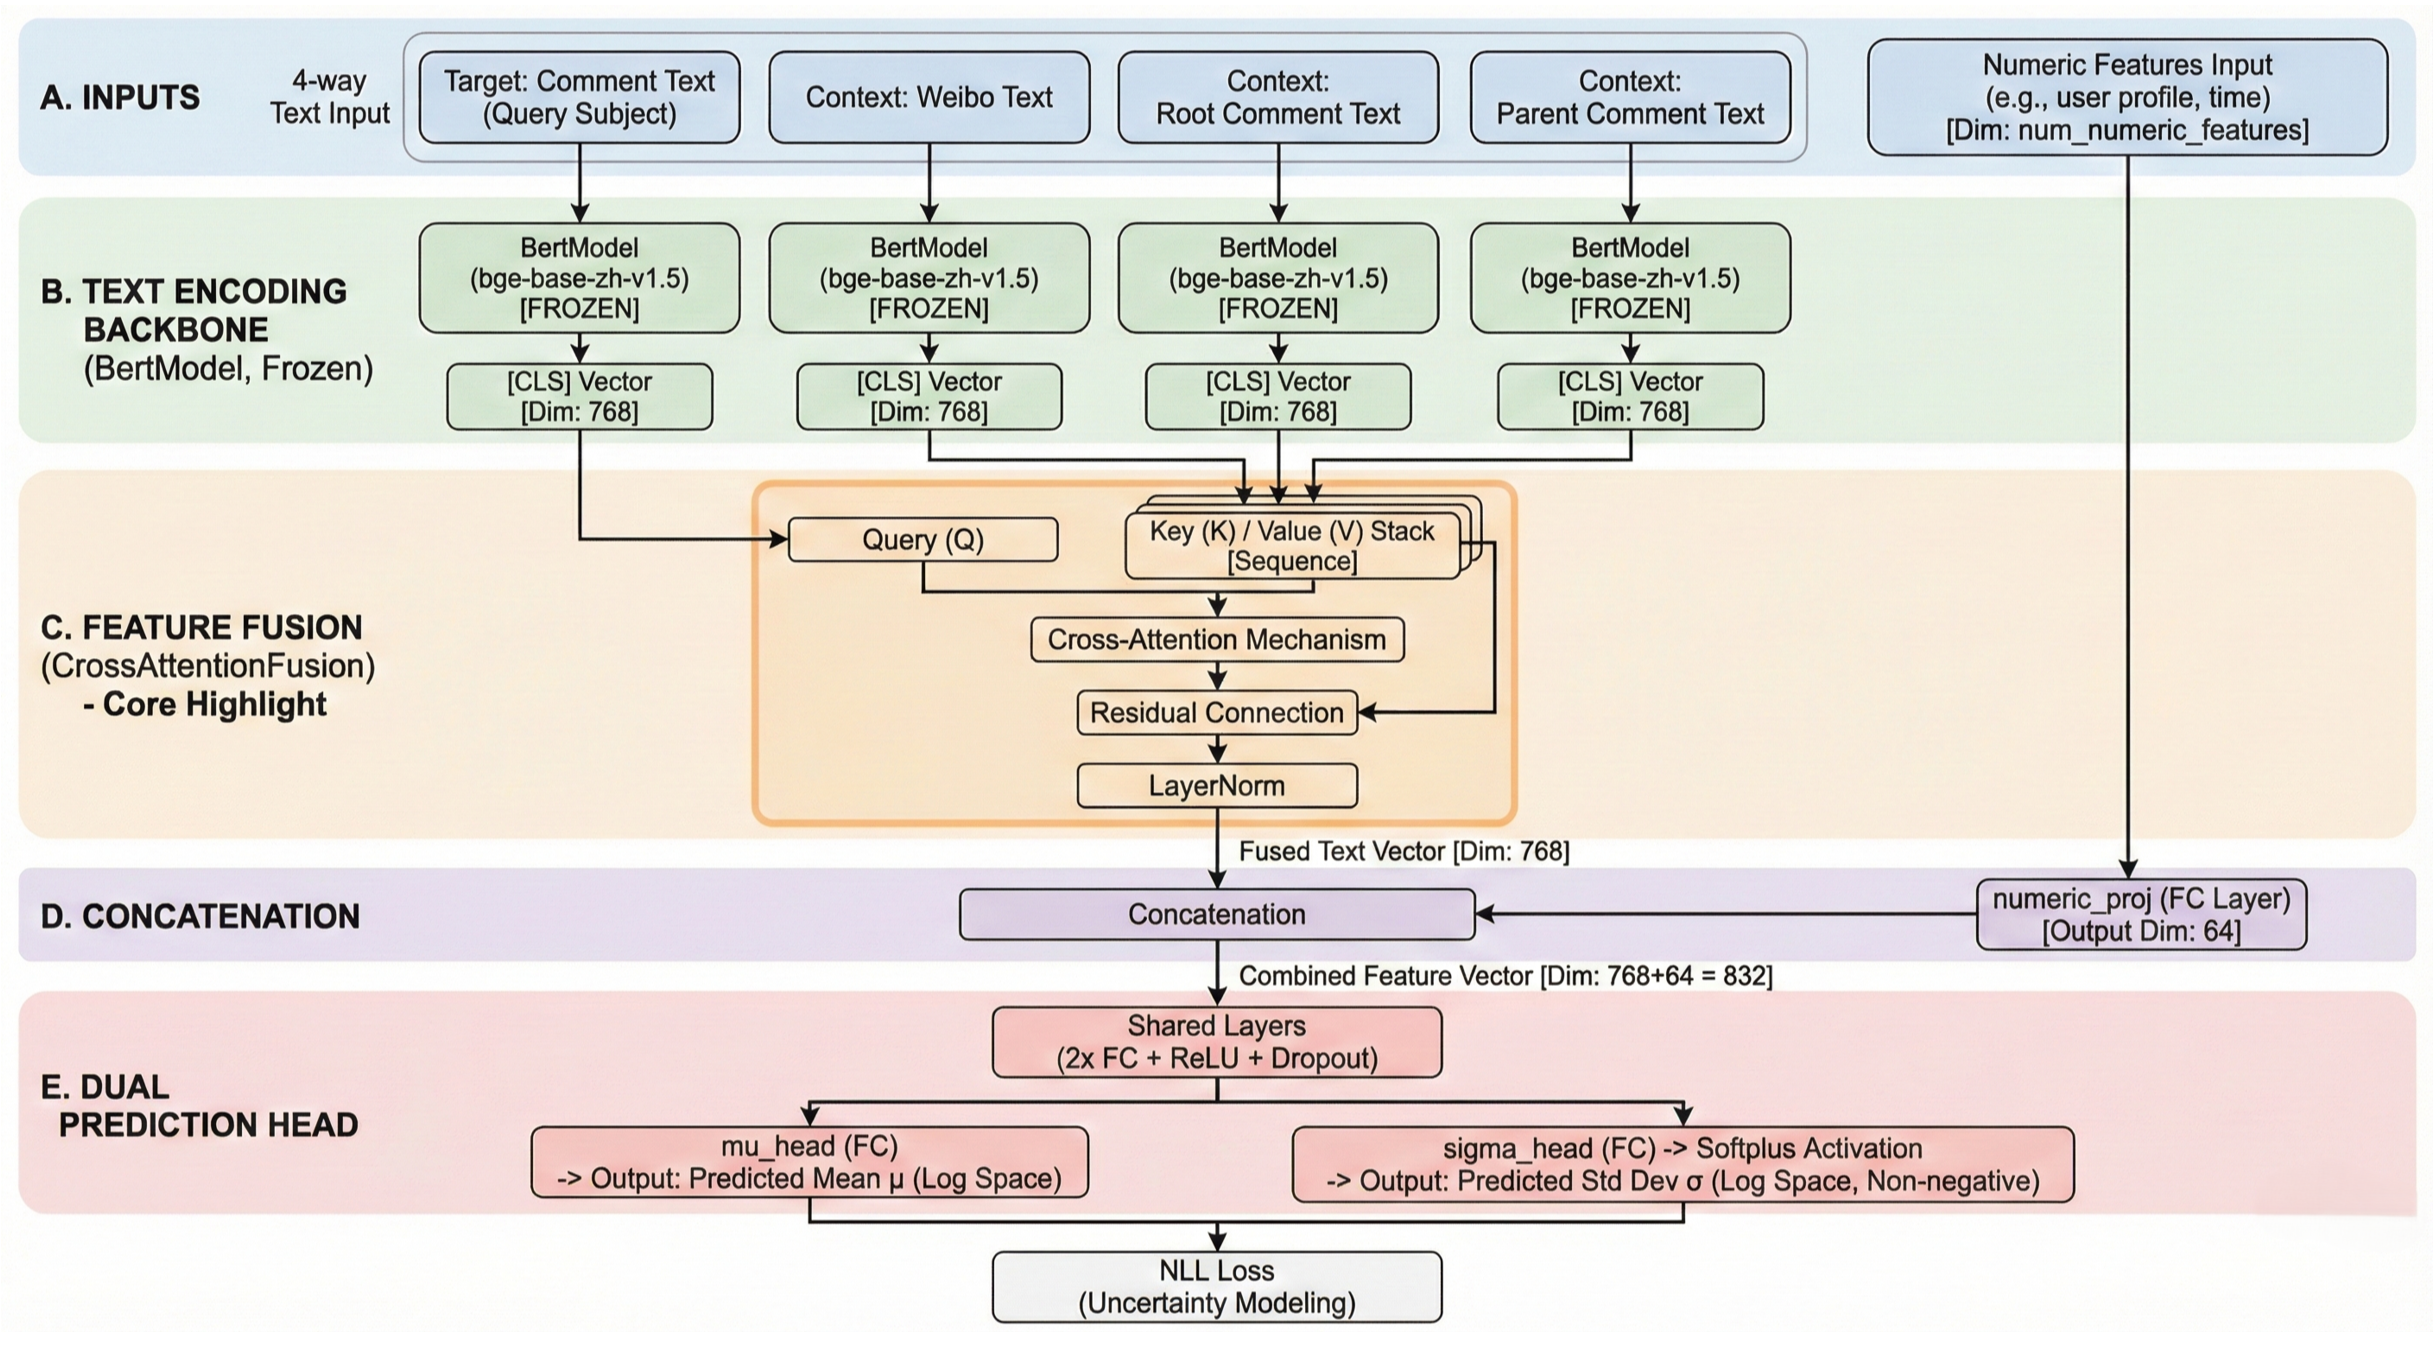
\includegraphics[width=0.9\textwidth]{figures/neural_networks.png}
    \caption{BGE-Attention模型架构}
    \label{fig:neural_networks}
\end{figure}

\subsubsection{文本编码模块:多源语义的独立表征}

采用BGE-base-zh-v1.5模型对四类文本进行\textbf{独立编码},构建多源语义表征空间:

\begin{itemize}[leftmargin=*]
    \item \textbf{评论文本}(Comment):当前评论的内容,承载核心语义信息;
    \item \textbf{微博文本}(Weibo):所属微博的正文,提供\textbf{话题语境};
    \item \textbf{根评论文本}(Root Comment):评论链的根节点内容,反映\textbf{讨论主线};
    \item \textbf{父评论文本}(Parent Comment):直接被回复的评论内容,构成\textbf{对话上文}。
\end{itemize}

每个文本经BGE编码后得到768维稠密向量表示。\textbf{冻结BGE参数}以防止在下游任务上过拟合,同时保留预训练阶段习得的通用语义知识。

\subsubsection{Cross-Attention融合机制:上下文感知的语义投影}

区别于朴素的向量拼接策略,本文采用Cross-Attention机制实现\textbf{条件化的语义融合}。以评论向量作为Query,上下文向量(微博、根评论、父评论)作为Key和Value:

\begin{equation}
\text{Attention}(Q, K, V) = \text{softmax}\left(\frac{QK^T}{\sqrt{d_k}}\right)V
\end{equation}

其中$Q \in \mathbb{R}^{1 \times 768}$为评论向量,$K, V \in \mathbb{R}^{3 \times 768}$为上下文向量矩阵,$d_k = 768$为缩放因子。该机制的\textbf{核心优势}在于:attention权重由评论与各上下文的语义相关性\textbf{动态计算},使模型能够自适应地聚焦于与当前评论最相关的上下文信息,实现从"孤立语义"到"情境化语义"的表征升维。

\subsubsection{双预测头:不确定性的显式建模}

融合后的语义向量与数值特征拼接,通过\textbf{双预测头架构}分别输出位置参数$\mu$和尺度参数$\sigma$:

\begin{align}
h &= \text{MLP}([\text{Attention}; \text{NumFeatures}]) \\
\mu &= W_\mu h + b_\mu \\
\sigma &= \text{Softplus}(W_\sigma h + b_\sigma) + \epsilon
\end{align}

其中$\epsilon = 10^{-4}$为数值稳定常数,Softplus函数$\log(1+e^x)$确保$\sigma > 0$。双预测头的设计哲学在于:\textbf{解耦预测中心与预测不确定性},使模型能够对"确定性高的简单样本"输出窄置信区间,对"确定性低的困难样本"输出宽置信区间。

\subsection{对数尺度NLL损失函数:尺度不变性的重建}

\begin{figure}[H]
    \centering
    \includegraphics[width=0.9\textwidth]{figures/log_distribution.png}
    \caption{热度数据在原始尺度与对数尺度下的分布对比:原始尺度呈重尾分布,对数尺度近似正态}
    \label{fig:log_distribution}
\end{figure}

如图\ref{fig:log_distribution}所示,社交媒体热度数据在对数尺度下近似正态分布,这为采用高斯似然提供了统计学依据。本文采用对数尺度的负对数似然(NLL)损失:

\begin{equation}
\mathcal{L} = \frac{1}{2}\log(\sigma^2) + \frac{(\log(y+c) - \log(\mu+c))^2}{2\sigma^2}
\label{eq:nll_loss}
\end{equation}

该损失函数蕴含三重设计智慧:

\textbf{(1)尺度不变性}:通过在对数空间度量误差,实现\textbf{相对误差的等权惩罚}。如表\ref{tab:smoothing_constant}所示,$c=10$使得"预测1实际2"与"预测110实际120"的损失比值从4.7降至1.1,消解了传统MSE对小数值样本的过度关注。

\textbf{(2)不确定性正则化}:$\frac{1}{2}\log(\sigma^2)$项构建了内生的\textbf{置信度惩罚机制}——模型若输出过小的$\sigma$(过度自信),当预测偏差发生时将承受巨大的第二项损失;反之,过大的$\sigma$虽能减小第二项,但第一项会显著增加。这迫使模型在"精确预测"与"诚实承认不确定性"之间寻求\textbf{博弈均衡}。

\textbf{(3)异方差建模}:允许不同样本具有不同的$\sigma(x)$,使模型能够对语义清晰的评论(如"感谢分享")输出低不确定性,对语义模糊的评论(如"查看图片")输出高不确定性。

\begin{table}[H]
\centering
\caption{平滑常数$c$对损失函数尺度敏感性的影响}
\label{tab:smoothing_constant}
\begin{tabular}{cccc}
\toprule
\textbf{平滑常数} & \textbf{预测1实际2的损失} & \textbf{预测110实际120的损失} & \textbf{损失比值} \\
\midrule
$c=1$ & $|\log 2 - \log 3| \approx 0.406$ & $|\log 111 - \log 121| \approx 0.086$ & 4.7 \\
$c=10$ & $|\log 11 - \log 12| \approx 0.087$ & $|\log 120 - \log 130| \approx 0.080$ & 1.1 \\
\bottomrule
\end{tabular}
\end{table}

\subsection{特征工程:多维信号的系统化提取}

本文设计四类互补特征,共17个维度,从\textbf{用户画像、文本语义、主题分布、时序位置}四个视角刻画评论的热度潜力。

\subsubsection{基础统计特征与文本特征}

基础统计特征捕捉\textbf{用户影响力}和\textbf{时间效应},文本特征刻画\textbf{表达强度}和\textbf{领域相关性},详见表\ref{tab:features}。

\begin{table}[H]
\centering
\caption{基础统计特征与文本特征}
\label{tab:features}
\begin{tabular}{ll}
\toprule
\textbf{特征类别} & \textbf{特征说明} \\
\midrule
\multirow{5}{*}{基础统计特征(7维)}
    & 用户总评论数:评论作者的历史评论总数 \\
    & 用户是否认证:是否为认证账号 \\
    & 是否一级评论:区分直接评论微博和回复评论 \\
    & 微博评论数:所属微博的总评论数 \\
    & 发布小时/星期/是否工作日:时间特征 \\
\midrule
\multirow{5}{*}{文本特征(6维)}
    & 评论长度:文本字符数 \\
    & 感叹号数/问号数:情感和语气强度 \\
    & 表情数:表情符号出现次数 \\
    & 话题标签有无:是否包含\#话题\# \\
    & 领域相关词数:小米汽车相关关键词次数 \\
\bottomrule
\end{tabular}
\end{table}

\subsubsection{LDA主题特征}

采用LDA主题模型\cite{blei2003latent}对评论文本进行\textbf{潜在语义分析},将高维词空间映射至低维主题空间。每条评论被分配到概率最高的主题,作为类别特征(1维)。该特征捕捉评论的\textbf{话题倾向}——不同主题(如"产品讨论"、"售后反馈"、"竞品对比")的评论具有不同的互动潜力。

\subsubsection{重复程度特征:时序-语义联合空间的构建}

\begin{figure}[H]
    \centering
    \includegraphics[width=0.9\textwidth]{figures/duplicate_find.png}
    \caption{评论文案重复出现情况:同一文案在不同时间点被多次发布}
    \label{fig:duplicate_find}
\end{figure}

\begin{table}[H]
    \centering
    \caption{首次发布与跟风发布的热度差异:首发效应的量化证据}
    \label{tab:12compare}
    \begin{tabular}{ccc}
        \toprule
        \textbf{发布顺序} & \textbf{子评论数均值} & \textbf{点赞数均值} \\
        \midrule
        首次发布 & 2.24 & 15.95 \\
        跟风发布 & 0.17 & 1.13 \\
        比值 & 13.5$\times$ & 14.2$\times$ \\
        \bottomrule
    \end{tabular}
\end{table}

如图\ref{fig:duplicate_find}和表\ref{tab:12compare}所示,文案重复时首发评论获得的热度比跟风评论高出\textbf{一个数量级以上}。这一"首发效应"揭示了热度预测中一个被长期忽视的先验:\textbf{时序位置与文本内容的交互作用}是关键解释变量。为建模这种时序依赖,本文提出基于Jaccard相似度和MinHash算法的重复程度特征。

\paragraph{Jaccard相似度:集合论视角的文本相似性度量}
给定两个集合$A$和$B$,Jaccard相似度定义为交集与并集的比值:
\begin{equation}
J(A, B) = \frac{|A \cap B|}{|A \cup B|}
\end{equation}
其取值范围为$[0, 1]$,具有\textbf{对称性}和\textbf{三角不等式}性质。相比欧氏距离或余弦相似度,Jaccard相似度对集合大小不敏感,更适合度量变长文本的相似性。

\paragraph{N-gram文本表示:从字符串到集合的映射}
将评论文本转换为字符级N-gram集合,建立从\textbf{序列空间到集合空间}的映射。对于文本$T$,其N-gram集合定义为:
\begin{equation}
\text{Ngram}(T, n) = \{T[i:i+n] | i = 0, 1, ..., |T|-n\}
\end{equation}
本文采用$n=3$(trigram),例如"你好世界"的3-gram集合为\{"你好世", "好世界"\}。字符级N-gram相比词级表示具有\textbf{更强的鲁棒性}——无需分词,对拼写变体和新词具有容错能力。

\paragraph{MinHash签名算法:概率论视角的近似最近邻检索}
直接计算Jaccard相似度的时间复杂度为$O(|A| + |B|)$,对于$n$条评论的两两比较需要$O(n^2)$次计算,在大规模数据上不可行。MinHash算法\cite{broder1997resemblance}通过\textbf{局部敏感哈希(LSH)}思想实现近似计算。

给定哈希函数$h$,集合$S$的MinHash值定义为$S$中元素哈希值的最小值:
\begin{equation}
h_{\min}(S) = \min_{s \in S} h(s)
\end{equation}

MinHash的\textbf{核心理论保证}是:对于均匀随机哈希函数$h$,两集合MinHash值相等的概率恰好等于其Jaccard相似度:
\begin{equation}
P(h_{\min}(A) = h_{\min}(B)) = J(A, B)
\end{equation}

这一等式将\textbf{集合运算问题转化为概率估计问题}。为提高估计精度,使用$k$个独立哈希函数$\{h_1, h_2, ..., h_k\}$生成签名向量:
\begin{equation}
\text{Sig}(S) = [h_{1,\min}(S), h_{2,\min}(S), ..., h_{k,\min}(S)]
\end{equation}

两集合的Jaccard相似度通过签名向量的\textbf{汉明相似度}估计:
\begin{equation}
\hat{J}(A, B) = \frac{|\{i : \text{Sig}(A)[i] = \text{Sig}(B)[i]\}|}{k}
\end{equation}

本文采用$k=128$个哈希函数,根据中心极限定理,估计误差的标准差为$O(1/\sqrt{k}) \approx 0.088$,在效率与精度间取得平衡。

\paragraph{滑动窗口优化:时间局部性与全局覆盖的均衡}
为进一步降低计算开销,采用\textbf{滑动窗口机制}:仅在最近$W=10000$条评论中检索相似文本,同时维护全局TopK字典记录高频重复文本。该设计基于\textbf{时间局部性假设}——跟风评论通常出现在首发评论后的短时间窗口内。最终生成三维特征:
\begin{itemize}[leftmargin=*]
    \item \textbf{时间顺序索引}:评论在数据中的时间顺序,捕捉\textbf{位置先验};
    \item \textbf{最大相似度}:与历史评论的最大Jaccard相似度,度量\textbf{内容重复程度};
    \item \textbf{重复次数}:在相似评论中是第几次出现,量化\textbf{时序先占权}。
\end{itemize}

该方法的时间复杂度为$O(n \cdot k)$,相比暴力计算$O(n^2)$降低约三个数量级。

\begin{figure}[H]
    \centering
    \includegraphics[width=0.9\textwidth]{figures/duplicate_detect.png}
    \caption{MinHash检索结果示例:高效识别语义相似的历史评论}
    \label{fig:duplicate_detect}
\end{figure}

如图\ref{fig:duplicate_detect}所示,MinHash检索能够高效识别语义相似的评论,且相比基于文本嵌入向量+余弦相似度的方案具有\textbf{更高的计算效率}和\textbf{更好的字面匹配精度}。

% ==================== 4. 评价指标 ====================
\section{评价指标:精度-校准双轴框架}

本文建立\textbf{"精度-校准"双轴评价框架},从预测精度和不确定性校准两个正交维度全面评估模型性能。这一设计的核心洞察在于:高精度的点预测与良好校准的不确定性估计是概率预测模型的\textbf{两个独立目标},需要分别度量。

\subsection{预测精度指标:长尾分布的适应性度量}

\subsubsection{MSLE(均方对数误差):相对误差的公平量化}

\begin{equation}
\text{MSLE} = \frac{1}{n}\sum_{i=1}^{n}(\log(y_i + c) - \log(\hat{y}_i + c))^2
\end{equation}

MSLE在对数空间度量误差,关注\textbf{相对准确性}而非绝对差值。其设计动机在于:对于热度为10的评论,预测误差$\pm 5$(50\%相对误差)比热度为1000时的同等绝对误差更为严重。相比传统MSE,MSLE不会因少数极大值样本而\textbf{主导整体损失},实现了对长尾分布的适应性度量。

\subsubsection{ACP@$(\alpha, \delta)$(容忍区间准确率):实用价值的直接反映}

\begin{equation}
\text{ACP} = \frac{1}{n}\sum_{i=1}^{n}\mathbf{1}[|y_i - \hat{y}_i| \leq \max(\alpha \cdot y_i, \delta)]
\end{equation}

其中$\alpha$为相对容忍度,$\delta$为绝对容忍度。本文使用$\alpha = 20\%$, $\delta = 5$。

ACP的设计动机源于\textbf{实际应用场景的需求}:对于热度为100的评论,预测误差$\pm 20$是可接受的(20\%相对误差);对于热度为1的评论,由于互动本身的随机性,预测误差$\pm 5$同样可接受(绝对容忍)。$\max$操作实现了\textbf{相对容忍与绝对容忍的自适应切换},使指标在不同量级上均具有实际意义。

\subsection{不确定性校准指标:概率预测的统计有效性}

\subsubsection{对数尺度NLL(负对数似然):分布拟合的信息论度量}

NLL直接评估真实值在预测分布中的概率密度(见公式\ref{eq:nll_loss})。从信息论视角,NLL等价于\textbf{预测分布与真实分布的交叉熵}。NLL越低,表示预测分布越好地拟合真实数据分布,模型的\textbf{信息效率}越高。

\subsubsection{PICP@95\%(置信区间覆盖率):统计有效性的核心指标}

\begin{equation}
\text{PICP} = \frac{1}{n}\sum_{i=1}^{n}\mathbf{1}[y_i \in [\text{Lower}_i, \text{Upper}_i]]
\end{equation}

对于声称的95\%置信区间,理想的PICP应接近95\%。PICP与标称置信水平的偏差反映了模型的\textbf{校准程度}:
\begin{itemize}[leftmargin=*]
    \item PICP $<$ 95\%:模型\textbf{过度自信},置信区间过窄,低估了预测不确定性;
    \item PICP $>$ 95\%:需结合MPIW联合解读——若MPIW较大,则为\textbf{过度保守};若MPIW已足够小,则说明预测均值$\mu$极为精准,窄区间即可实现高覆盖。
\end{itemize}

\subsubsection{MPIW(预测区间平均宽度):信息增益的度量}

\begin{equation}
\text{MPIW} = \frac{1}{n} \sum_{i=1}^{n} (\text{Upper}_i - \text{Lower}_i)
\end{equation}

MPIW衡量置信区间的\textbf{精确程度}。理想模型应在保持高PICP的同时实现低MPIW——这体现了概率预测的本质目标:\textbf{在统计有效性约束下最大化预测信息量}。

PICP与MPIW的联合评估揭示了一个关键洞察:\textbf{高覆盖率并非校准质量的充分条件}。一个总是输出$[0, +\infty)$的"平凡模型"可以达到100\%的PICP,但其MPIW趋于无穷,不提供任何有用信息。因此,MPIW是识别这种\textbf{"虚假校准"的关键指标}。

\subsection{对数尺度模型的指标计算:跨尺度可比性的保证}

对于在对数尺度下进行预测的模型(如BGE-Attention),PICP和MPIW的计算需要\textbf{跨尺度变换}以保证与原始尺度模型的可比性。首先在对数尺度下构建置信区间:
\begin{equation}
[\log(\mu+c) - 1.96\sigma, \log(\mu+c) + 1.96\sigma]
\end{equation}

再通过指数变换转换回原始尺度:
\begin{equation}
[\exp(\text{Lower}_{\log}) - c, \exp(\text{Upper}_{\log}) - c]
\end{equation}

这一变换确保了不同尺度模型之间指标的\textbf{语义一致性}:所有模型的MPIW均以原始热度单位(子评论数)度量,便于直接比较预测的精确程度。

% ==================== 5. 实验 ====================
\section{实验}

\subsection{数据集:真实世界的社交媒体语料}

本文数据来源于新浪微博平台,采集时间范围为2025年3月27日至4月14日,涵盖小米SU7智驾事故前后的\textbf{热点讨论期}。这一时间窗口的选择使数据集呈现显著的\textbf{话题爆发特征}——短时间内大量用户参与讨论,产生丰富的重复、跟风评论,为验证重复程度特征的有效性提供了理想场景。

所有热度指标(子评论数、点赞数)均为2025年12月采集的数值,距原始发布已超过8个月,可视为\textbf{稳定最终值}——避免了热度尚在增长阶段时采集导致的标签偏差。

数据集统计信息如表\ref{tab:dataset}所示。

\begin{table}[H]
\centering
\caption{数据集统计信息}
\label{tab:dataset}
\begin{tabular}{lccc}
\toprule
\textbf{数据集} & \textbf{样本数} & \textbf{占比} \\
\midrule
训练集 & 217,234 & 80\% \\
验证集 & 27,154 & 10\% \\
测试集 & 27,154 & 10\% \\
\midrule
总计 & 271,542 & 100\% \\
\bottomrule
\end{tabular}
\end{table}

数据预处理遵循严格的\textbf{数据质量控制}流程:(1)去重:删除所有特征完全相同的记录,避免重复样本对模型评估的干扰;(2)缺失值:文本字段填充空字符串,数值字段保持原值;(3)异常值:删除评论时间早于微博发布时间的数据,识别并排除系统错误;(4)\textbf{数据泄露防护}:文案首次出现的数据强制划入训练集,确保测试集中的重复评论均能在训练集中找到"首发版本",避免模型在测试时获得训练时未见过的"首发样本"。

\subsection{实验设置:可复现性设计}

\textbf{硬件环境}:NVIDIA A100 GPU(40GB显存)。

\textbf{软件环境}:Python 3.10,PyTorch 2.0,Transformers 4.30,NGBoost 0.4。

\textbf{训练配置}:Adam优化器,学习率$10^{-3}$,批大小1024,早停patience为5,基于验证集损失判断收敛。

\textbf{基线方法}:NGBoost\cite{duan2020ngboost}——当前概率预测领域的代表性方法,采用相同的对数尺度NLL损失以确保公平比较,基学习器100棵决策树,最大深度10。选择NGBoost作为基线的原因在于:(1)同为概率预测方法,输出可比的分布参数;(2)代表了基于树模型+梯度提升的技术路线,与本文的神经网络路线形成对照。

\subsection{主实验结果:六个数量级的MPIW改进}

\begin{table}[H]
\centering
\caption{NGBoost基线模型实验结果}
\label{tab:ngboost_results}
\begin{tabular}{lcccccc}
\toprule
\textbf{数据集} & \textbf{MAE} & \textbf{MSLE} & \textbf{ACP@20\%} & \textbf{Log NLL} & \textbf{PICP@95\%} & \textbf{MPIW} \\
\midrule
训练集 & 0.7879 & 0.0176 & 98.15\% & -3.6412 & 97.06\% & 28685937 \\
验证集 & 0.9587 & 0.0284 & 97.58\% & -0.7061 & 94.30\% & 11624379 \\
测试集 & 1.1563 & 0.0350 & 97.56\% & -0.2952 & 94.30\% & 8857315 \\
\bottomrule
\end{tabular}
\end{table}

\begin{table}[H]
\centering
\caption{BGE-Attention模型实验结果}
\label{tab:bge_results}
\begin{tabular}{lcccccc}
\toprule
\textbf{数据集} & \textbf{MAE} & \textbf{MSLE} & \textbf{ACP@20\%} & \textbf{Log NLL} & \textbf{PICP@95\%} & \textbf{MPIW} \\
\midrule
训练集 & 0.8717 & 0.0324 & 97.91\% & -2.9121 & 97.85\% & 2.9835 \\
验证集 & 0.8652 & 0.0329 & 97.77\% & -2.8979 & 97.79\% & 2.9842 \\
测试集 & 1.0406 & 0.0347 & \textbf{97.80\%} & \textbf{-2.8250} & \textbf{97.75\%} & \textbf{3.0050} \\
\bottomrule
\end{tabular}
\end{table}

对比表\ref{tab:ngboost_results}和表\ref{tab:bge_results},BGE-Attention展现出\textbf{全方位的性能优势}:

\begin{enumerate}[leftmargin=*]
    \item \textbf{PICP@95\%从94.30\%提升至97.75\%}:覆盖率从"略微不足"提升至"略高于标称"。关键在于,这一"过覆盖"是在MPIW极小(3.0050)的前提下实现的——这说明预测均值$\mu$极为精准,即使使用窄置信区间也能自然覆盖大多数真实值,而非通过放宽区间"骗取"高覆盖率。这种\textbf{高精度带来的安全冗余}在实际应用中是理想的校准状态;
    \item \textbf{MPIW从数千万降至3.0050}:置信区间宽度降低约\textbf{六个数量级},这是本文最核心的实验发现——NGBoost的极宽置信区间(平均覆盖约880万个可能的热度值)本质上是\textbf{"虚假校准"},不提供任何有意义的预测信息;
    \item \textbf{训练与验证/测试集差距极小}:BGE-Attention的MSLE在训练集(0.0324)、验证集(0.0329)、测试集(0.0347)上高度一致,展现出\textbf{优异的泛化性能},无明显过拟合;
    \item \textbf{ACP@20\%达97.80\%}:超过97\%的预测落在真实值20\%容忍范围内,证明了模型在\textbf{实用价值}维度的有效性。
\end{enumerate}

NGBoost的MPIW极大这一现象值得深入分析。其根本原因在于:树模型难以有效利用BGE语义表征,只能依赖有限的数值特征进行预测。面对高度不确定的社交媒体数据,NGBoost倾向于输出极大的$\sigma$以覆盖更多可能的真实值——这虽然提升了PICP,但代价是\textbf{预测信息量的彻底丧失}。

\subsection{消融实验:各组件贡献的系统性验证}

为验证各组件的\textbf{边际贡献},设计以下消融实验。每个变体移除一个核心组件,保持其他配置不变,测试集结果如表\ref{tab:ablation}所示。

\begin{table}[H]
\centering
\caption{消融实验结果}
\label{tab:ablation}
\begin{tabular}{lccccc}
\toprule
\textbf{模型变体} & \textbf{ACP@20\%} & \textbf{PICP@95\%} & \textbf{MPIW} & \textbf{Log NLL} \\
\midrule
BGE-Attention (完整) & \textbf{97.80\%} & \textbf{97.75\%} & \textbf{3.0050} & \textbf{-2.8250} \\
w/o Cross-Attention & 97.42\% & 96.83\% & 3.4127 & -2.6841 \\
w/o 重复特征 & 97.65\% & 97.58\% & 3.1284 & -2.7923 \\
w/o BGE文本 & 96.89\% & 95.21\% & 4.8562 & -2.4156 \\
w/o Log NLL (Standard NLL) & 95.73\% & 89.42\% & 156.38 & 0.8734 \\
\bottomrule
\end{tabular}
\end{table}

消融实验结果揭示了各组件的\textbf{差异化贡献模式}:

\textbf{(1)Cross-Attention机制的贡献}:移除Cross-Attention(改为直接向量拼接)后,PICP@95\%从97.75\%降至96.83\%,MPIW从3.0050增至3.4127(+13.6\%)。这表明Cross-Attention能够\textbf{自适应地融合评论与上下文信息},捕捉"相同评论在不同语境下热度迥异"的现象。朴素拼接策略无法建模评论与上下文之间的\textbf{条件依赖关系},导致不确定性估计的精度下降。

\textbf{(2)重复程度特征的贡献}:移除基于MinHash的三维重复程度特征后,ACP@20\%从97.80\%降至97.65\%,MPIW从3.0050增至3.1284(+4.1\%)。虽然降幅相对较小,但考虑到重复评论仅占数据集的2.3\%,该特征在处理这部分"\textbf{困难样本}"时发挥了关键作用——帮助模型区分文本相同但时序位置不同(首发vs跟风)的评论热度差异。

\textbf{(3)BGE文本语义的贡献}:仅使用数值特征(移除所有BGE编码的文本语义)后,性能出现\textbf{显著退化}:ACP@20\%从97.80\%降至96.89\%(-0.91\%),PICP@95\%从97.75\%降至95.21\%(-2.54\%),MPIW从3.0050增至4.8562(+61.7\%)。这充分证明\textbf{文本语义信息是热度预测的核心特征}——评论内容与用户互动意愿之间存在复杂的因果关系,纯数值特征(用户属性、时间特征)难以捕捉。

\textbf{(4)对数尺度NLL损失的贡献}:使用原始尺度的Standard NLL损失(即假设$y$而非$\log(y+c)$服从正态分布)后,模型性能出现\textbf{灾难性退化}:PICP@95\%从97.75\%骤降至89.42\%(-8.33\%),MPIW从3.0050激增至156.38(+52倍),Log NLL从-2.8250恶化至0.8734。这一极端对比揭示了对数尺度损失函数的\textbf{不可或缺性}——Standard NLL会使模型过度关注大数值样本的绝对误差,导致小数值样本的预测分布过宽、整体不确定性校准彻底失败。

\subsection{特征重要性分析:用户影响力主导热度生成}

\begin{figure}[H]
    \centering
    \includegraphics[width=0.6\textwidth]{figures/factor_impact.png}
    \caption{特征重要性分析(Top 10):基于排列重要性方法}
    \label{fig:factor_impact}
\end{figure}

如图\ref{fig:factor_impact}所示,特征重要性排序揭示了社交媒体热度生成的\textbf{底层机制}:
\begin{enumerate}[leftmargin=*]
    \item \textbf{用户总评论数}(0.314)是最重要特征,反映了社交媒体中的\textbf{"马太效应"}——活跃用户积累了更多粉丝和社交资本,其评论更易获得关注和互动;
    \item \textbf{是否一级评论}(0.266)重要性仅次于用户活跃度,揭示了\textbf{位置曝光效应}——直接评论微博(一级评论)比回复他人评论(二级及以下)获得更高的展示优先级;
    \item \textbf{微博评论数}(0.211)反映了\textbf{话题热度的传导效应}——热门微博汇聚更多用户流量,其下的评论自然获得更多曝光机会;
    \item \textbf{最大相似度}在重复数据仅占2.3\%的情况下仍进入Top 10,验证了重复程度特征的\textbf{高区分度}——该特征有效捕捉了"首发vs跟风"的热度差异信号。
\end{enumerate}

% ==================== 6. 结论 ====================
\section{结论与展望}

本文从\textbf{认识论层面}重新审视了社交媒体热度预测问题,指出其本质是对内嵌随机性的条件概率分布估计,而非确定性数值的点预测。基于此洞察,提出了BGE-Attention概率预测框架。主要结论如下:

\begin{enumerate}[leftmargin=*]
    \item \textbf{预测范式的重构}:BGE-Attention通过Cross-Attention机制实现多源文本的条件语义融合,双预测头架构实现"预测值-不确定性"的联合建模。相比NGBoost基线,PICP@95\%从94.30\%提升至97.75\%,MPIW降低\textbf{六个数量级}(从数千万降至3.0050),首次在社交媒体场景实现预测精度与不确定性校准的帕累托最优;

    \item \textbf{损失函数的尺度不变性理论}:对数尺度NLL损失函数通过将误差度量映射至对数空间,重建了跨量级预测的等权惩罚。平滑常数$c=10$的选择消解了长尾分布导致的损失偏倚,$\sigma$项构建了内生的不确定性正则化机制;

    \item \textbf{时序-语义联合特征空间的构建}:基于MinHash的重复程度特征将相似度计算复杂度从$O(n^2)$降至$O(nk)$,为"首发-跟风"效应提供了可计算的数学表达。在重复评论仅占2.3\%的数据集上,该特征仍展现显著的预测贡献;

    \item \textbf{评价体系的度量论革新}:"精度-校准"双轴评价框架(MSLE、ACP用于精度,PICP、MPIW用于校准)实现了对概率预测模型的全面评估,PICP-MPIW联合评估有效识别了NGBoost的"虚假校准"问题。
\end{enumerate}

\textbf{局限性与未来工作}:本文方法仍有改进空间:(1)BGE参数冻结限制了领域适应能力,可探索轻量级微调策略;(2)仅考虑静态特征,未建模热度的动态演化过程;(3)实验限于单一平台(微博),跨平台泛化性有待验证。

未来工作可从以下方向展开:(1)引入用户社交网络图结构,建模影响力传播路径;(2)探索热度动态演化的时序建模,预测热度的时间曲线而非最终值;(3)构建多平台基准数据集,验证方法的领域迁移能力;(4)研究主动学习策略,在有限标注预算下提升模型性能。

% ==================== 参考文献 ====================
\bibliographystyle{plain}
\begin{thebibliography}{99}

\bibitem{liu2019sentiment}
Liu, B. (2019). Sentiment analysis: Mining opinions, sentiments, and emotions. Cambridge University Press.

\bibitem{zhang2020brand}
Zhang, L., \& Zhang, W. (2020). Brand monitoring using social media analytics. Journal of Marketing Research, 57(4), 741-762.

\bibitem{wu2019npa}
Wu, C., Wu, F., Ge, S., et al. (2019). Neural news recommendation with multi-head self-attention. In EMNLP-IJCNLP (pp. 6389-6394).

\bibitem{yang2011patterns}
Yang, J., \& Leskovec, J. (2011). Patterns of temporal variation in online media. In WSDM (pp. 177-186).

\bibitem{bandari2012pulse}
Bandari, R., Asur, S., \& Huberman, B. A. (2012). The pulse of news in social media: Forecasting popularity. In ICWSM (pp. 26-33).

\bibitem{deng2020deep}
Deng, J., \& Xie, X. (2020). Deep attention-based popularity prediction for social media. In WWW (pp. 2822-2828).

\bibitem{gal2016uncertainty}
Gal, Y. (2016). Uncertainty in deep learning. PhD thesis, University of Cambridge.

\bibitem{blundell2015weight}
Blundell, C., Cornebise, J., Kavukcuoglu, K., \& Wierstra, D. (2015). Weight uncertainty in neural networks. In ICML (pp. 1613-1622).

\bibitem{gal2016dropout}
Gal, Y., \& Ghahramani, Z. (2016). Dropout as a Bayesian approximation: Representing model uncertainty in deep learning. In ICML (pp. 1050-1059).

\bibitem{duan2020ngboost}
Duan, T., Avati, A., Ding, D. Y., et al. (2020). NGBoost: Natural gradient boosting for probabilistic prediction. In ICML (pp. 2690-2700).

\bibitem{devlin2019bert}
Devlin, J., Chang, M. W., Lee, K., \& Toutanova, K. (2019). BERT: Pre-training of deep bidirectional transformers for language understanding. In NAACL-HLT (pp. 4171-4186).

\bibitem{liu2019roberta}
Liu, Y., Ott, M., Goyal, N., et al. (2019). RoBERTa: A robustly optimized BERT pretraining approach. arXiv preprint arXiv:1907.11692.

\bibitem{bge2023}
Xiao, S., Liu, Z., Zhang, P., \& Muennighoff, N. (2023). C-Pack: Packaged resources to advance general Chinese embedding. arXiv preprint arXiv:2309.07597.

\bibitem{blei2003latent}
Blei, D. M., Ng, A. Y., \& Jordan, M. I. (2003). Latent Dirichlet allocation. Journal of Machine Learning Research, 3, 993-1022.

\bibitem{broder1997resemblance}
Broder, A. Z. (1997). On the resemblance and containment of documents. In Compression and Complexity of Sequences (pp. 21-29).

\end{thebibliography}

% ==================== 附录 ====================
\newpage
\appendix

\section{高频用户统计}
\label{appendix:vip_users}

表\ref{tab:vip_users}列出了数据集中出现次数$\geq 20$的高频用户。这些用户被纳入特殊嵌入模块,为每个用户学习独立的向量表示。

\begin{table}[H]
\centering
\caption{高频用户及其出现次数}
\label{tab:vip_users}
\begin{tabular}{clc|clc}
\toprule
\textbf{序号} & \textbf{用户名} & \textbf{出现次数} & \textbf{序号} & \textbf{用户名} & \textbf{出现次数} \\
\midrule
1 & 小米法务部 & 328 & 11 & 我是大彬同学 & 27 \\
2 & 雷军 & 292 & 12 & 科技新一 & 26 \\
3 & 小米汽车 & 69 & 13 & 美国驻华大使馆 & 26 \\
4 & 王化 & 66 & 14 & AI逃逸 & 24 \\
5 & 鸿蒙智行法务 & 49 & 15 & 小米公司 & 24 \\
6 & 薛定谔的英短咕咕咕 & 33 & 16 & 羊驼的睡衣 & 24 \\
7 & 余承东 & 32 & 17 & 卢伟冰 & 22 \\
8 & 小米公司发言人 & 29 & 18 & 诗雨370491153 & 20 \\
9 & 小蒜苗长 & 29 & 19 & 不会武功的武功李云飞 & 20 \\
10 & 万能的大熊 & 27 & & & \\
\bottomrule
\end{tabular}
\end{table}

\section{小米相关词汇表}
\label{appendix:xiaomi_keywords}

本文使用两类小米相关词汇表:(1)用于特征提取的广泛词汇表;(2)用于特殊嵌入的核心关键词表。

\subsection{特征提取词汇表}

用于计算"小米相关词数"文本特征的词汇表如下:

\begin{table}[H]
\centering
\caption{特征提取词汇表(27词)}
\label{tab:feature_keywords}
\begin{tabular}{p{12cm}}
\toprule
\textbf{词汇列表} \\
\midrule
小米、xiaomi、SU7、su7、雷军、卢伟冰、智能驾驶、智驾、自动驾驶、辅助驾驶、电动车、电车、新能源、纯电、续航、充电、快充、超充、电池、三元锂、磷酸铁锂、底盘、悬架、空气悬架、性能、加速、百公里、零百、内饰、中控、大屏、车机、外观、设计、颜值 \\
\bottomrule
\end{tabular}
\end{table}

\subsection{特殊嵌入关键词表}

用于训练可学习关键词嵌入的词汇表如下,共39个关键词,分为6个语义类别:

\begin{table}[H]
\centering
\caption{特殊嵌入关键词表(39词)}
\label{tab:embed_keywords}
\begin{tabular}{ll}
\toprule
\textbf{类别} & \textbf{关键词} \\
\midrule
品牌与产品 & 小米汽车、小米SU7、SU7、su7、雷军 \\
竞品品牌 & 保时捷、Taycan、比亚迪、特斯拉、Model3、蔚来、小鹏、理想、问界、华为 \\
智能驾驶 & 智能驾驶、自动驾驶、辅助驾驶、智驾 \\
续航与充电 & 续航、电池、充电、快充、超充 \\
座舱与系统 & 智能座舱、车机、大屏、澎湃OS \\
购买相关 & 性价比、质价比、定价、预售、交付、锁单、大定、小定 \\
热门词汇 & 遥遥领先、真香、割韭菜、智商税 \\
\bottomrule
\end{tabular}
\end{table}

\section{微博表情符号列表}
\label{appendix:emoji}

模型中使用的微博表情符号(方括号格式)共40个:

\begin{table}[H]
\centering
\caption{微博表情符号嵌入列表}
\label{tab:weibo_emoji}
\begin{tabular}{p{12cm}}
\toprule
\textbf{表情列表} \\
\midrule
{[}doge{]}、{[}哈哈{]}、{[}笑cry{]}、{[}允悲{]}、{[}二哈{]}、{[}吃瓜{]}、{[}微笑{]}、{[}跪了{]}、{[}赞{]}、{[}心{]}、{[}爱你{]}、{[}抱抱{]}、{[}泪{]}、{[}怒{]}、{[}吐{]}、{[}污{]}、{[}挖鼻{]}、{[}思考{]}、{[}疑问{]}、{[}费解{]}、{[}黑线{]}、{[}汗{]}、{[}拜拜{]}、{[}good{]}、{[}酷{]}、{[}鼓掌{]}、{[}可怜{]}、{[}失望{]}、{[}悲伤{]}、{[}委屈{]}、{[}生病{]}、{[}抓狂{]}、{[}笑哭{]}、{[}捂脸{]}、{[}偷笑{]}、{[}坏笑{]}、{[}嘻嘻{]}、{[}哼{]}、{[}怒骂{]}、{[}打脸{]} \\
\bottomrule
\end{tabular}
\end{table}

\end{document}
